\chapter{Contesto aziendale}
\label{chap:Contesto-aziendale}


\section{VisioneImpresa}

VisioneImpresa è un'azienda con oltre quarant'anni di esperienza nel settore dell'\textit{Information Technology}. La sua attività è focalizzata sullo sviluppo di soluzioni \textit{software} per l'automazione e l'organizzazione di processi aziendali. In particolare, offre una gamma di strumenti \mygls{ERP}, sistemi integrati che permettono di gestire e coordinare in modo centralizzato le attività operative, dalla contabilità alla logistica, ottimizzando la gestione delle informazioni in un ambiente condiviso.

La sede si trova a Pernumia (PD), all'interno di un casolare ristrutturato nel cuore del territorio delle Terme Euganee ed ospita un \textit{team} di circa venti persone. VisioneImpresa opera prevalentemente nel Nord Est, ma con contatti che si estendono su tutto il territorio nazionale.

Nel 2016 è entrata a far parte del gruppo OfficeGroup, un \textit{network} di aziende orientate alla progettazione di \textit{software} gestionali avanzati. L'ingresso in questa rete ha favorito la crescita soprattutto grazie allo scambio di conoscenze e competenze con altre aziende andando a rafforzare la posizione di mercato.

Il 5 ottobre 2023, VisioneImpresa diventa una società \textit{benefit}, come viene indicato sul sito aziendale \footcite{site:vsh-sb}, non è stata una scelta imposta ma è arrivata attraverso un lungo e consapevole percorso.
Questa forma giuridica rappresenta le società che affiancano agli obiettivi di profitto anche attività che portano al beneficio comune. 

\begin{figure}[H]
    \centering
    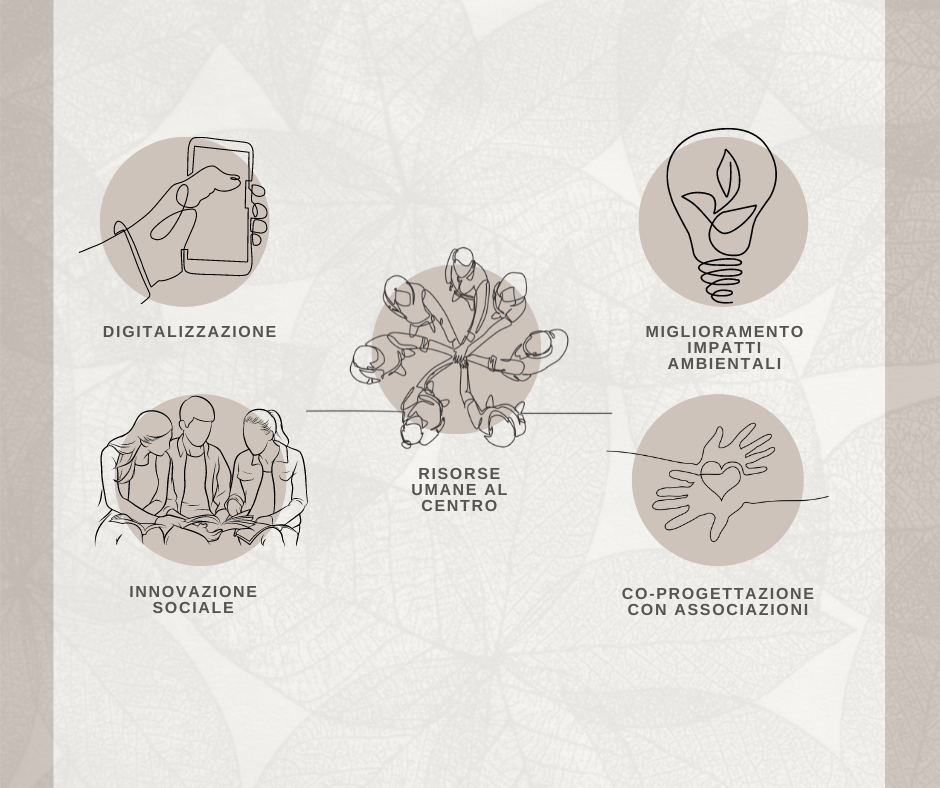
\includegraphics[alt={obiettivi società \textit{benefit}}, width=.5\columnwidth]{img/Sbenefit.png}
    \caption[Obiettivi di VisioneImpresa in quanto società \textit{benefit}.]{obiettivi di VisioneImpresa in quanto società \textit{benefit}. \\ \textit{fonte: \url{https://www.vsh.it/azienda/societa-benefit/}}}
    \label{fig:Benefit}
\end{figure} 

In qualità di società \textit{benefit} VisioneImpresa adotta una visione imprenditoriale responsabile, sostenibile e trasparente; assumendo impegni verso la società e l'ambiente.

Come dimostra la figura \ref{fig:Benefit} si impegna a perseguire i seguenti obiettivi:
\begin{itemize}
    \item La promozione della digitalizzazione al fine anche dell'utilizzo di minore quantità di materiali supportando la transizione ecologica.
    \item Il miglioramento delle condizioni lavorative, mettendo al centro il benessere delle risorse umane, riponendo particolare attenzione a tematiche come la parità di genere, la formazione continua e la conciliazione tra attività lavorativa e vita privata.
    \item La promozione di progetti orientati all'innovazione e al benessere sociale favorendo la collaborazione con enti del territorio tra cui scuole e università.
    \item Partecipazione attiva in progetti locali, favorendo la collaborazione con enti del territorio per generare valore alla comunità.
    \item Mantenere un'alta attenzione all'impatto ambientale, impegnandosi nell'utilizzo di risorse energetiche pulite e riducendo l'impatto attraverso pratiche legate al consumo di risorse e alla gestione dei rifiuti.
\end{itemize}

% ----------------------------------------------------------------

\section{Clienti e servizi}

% -----------------------------------------------------------

VisioneImpresa si rivolge principalmente a realtà di piccole e medie dimensioni situate nel Nord Est, ma opera anche in regioni del Centro Italia e in Sardegna. La principale offerta si fonda su soluzioni gestionali configurabili in base alle esigenze specifiche del cliente, affiancate da servizi di supporto tecnico e di consulenza. 
Il prodotto principale dell'azienda è VisionENTERPRISE, un sistema \mygls{ERP} modulare progettato per adattarsi a praticamente tutti i contesti aziendali.

\begin{figure}[H]
    \centering
    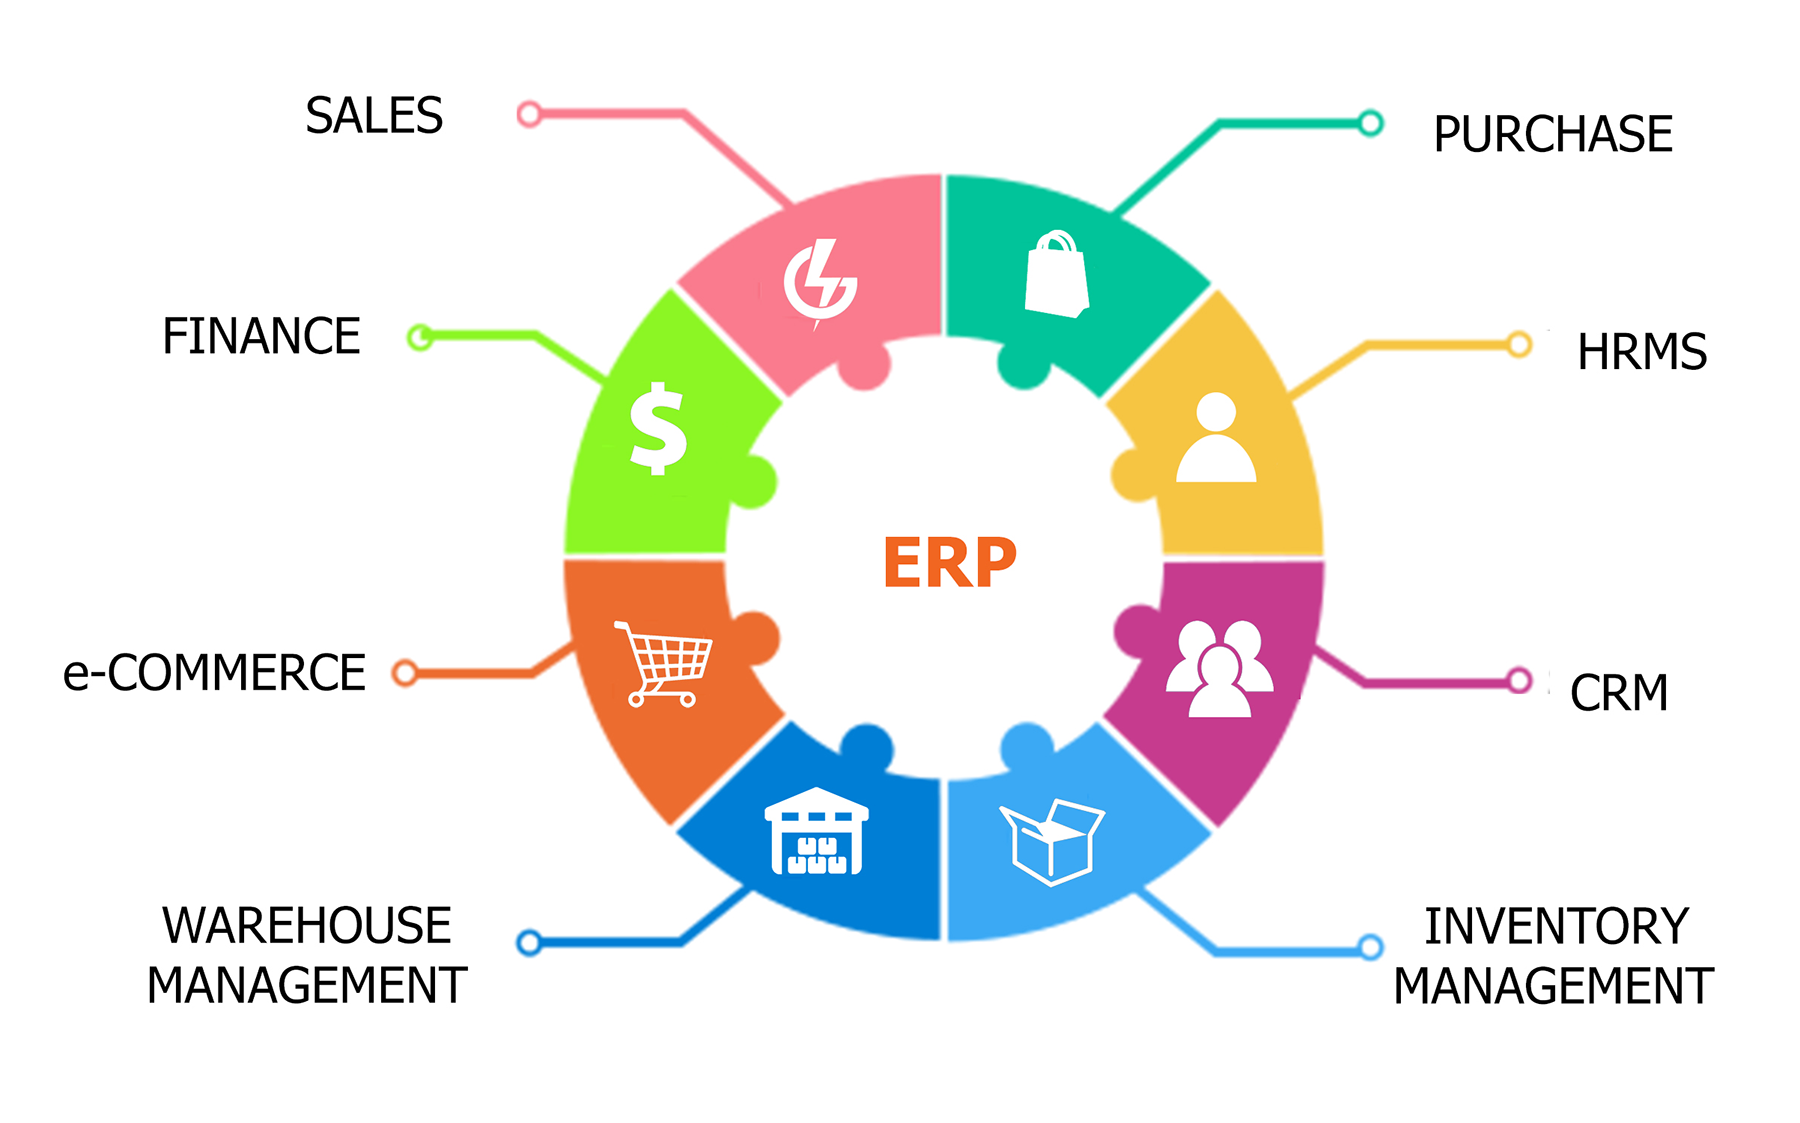
\includegraphics[alt={Enterprise Resource Planning}, width=1\columnwidth]{img/software-erp.png}
    \caption[Enterprise Resource Planning.]{Enterprise Resource Planning. \\ \textit{fonte: \url{https://www.softplaceweb.com/erp-open-source/}}}
    \label{fig:ERP}
\end{figure} 

Si tratta di un sistema flessibile, che costituisce una base alla quale vengono affiancate anche soluzioni verticali pensate per settori specifici. Questi prodotti verticali si basano sulla stessa infrastruttura \textit{software}, ma dispongono di funzionalità specifiche che hanno l'obiettivo di soddisfare esigenze particolari di determinate filiere produttive. \\


\textbf{Soluzioni verticali della linea Vision}\\
Le soluzioni verticali offerte da VisioneImpresa includono:
\begin{itemize}
\item \textbf{VisionENERGY:} Gestionale pensato per aziende del settore petrolifero, include diverse funzionalità, in aggiunta a quelle tipiche di un \mygls{ERP}, mirate a soddisfare bisogni di questo settore come la gestione della vendita del carburante, la manutenzione degli impianti, la fatturazione con defiscalizzazione e la manutenzione degli impianti.


\item \textbf{VisionBLUE:} Gestionale pensato per la filiera ittica, fornisce strumenti per attività legate alla vendita all'ingrosso dei prodotti ittici, come la gestione della tracciabilità dei prodotti, funzioni per l'inventario e organizzazione in contesti di alta intensità.


\item \textbf{VisionASSISTANCE:} Gestionale dedicato alle aziende che forniscono assistenza su prodotti, consente di gestire richieste di intervento, stipulazione di contratti di assistenza, organizzazione dei tecnici sul territorio e assegnazione di interventi.

\item \textbf{VisionFRESH:} Prodotto ideato per risolvere le esigenze del settore ortofrutticolo, contiene funzionalità che si integrano con le bilance elettriche, gestione dei lotti, imballaggi e prodotti e movimentazione della merce. 

\item \textbf{VisionANTINCENDI:} Gestionale che va a risolvere le richieste specifiche del settore della sicurezza e manutenzione di sistemi antincendio, offre funzionalità per la gestione degli interventi, gestione dei buoni di manutenzione e gestione dei contratti.


\item \textbf{VisionTRASPORTI:} Gestionale orientato alle aziende di logistica e trasporti, contiene funzionalità specifiche per facilitare la gestione dei listini, delle anagrafiche oppure funzionalità per la pianificazione dei tragitti.

\item \textbf{VisionELETTRO:} Gestionale dedicato alle officine elettromeccaniche, contiene funzionalità dedicate come la gestione delle matricole, gestione delle attività e navigazione per consultare lo storico degli interventi.

\end{itemize}

\textbf{Servizi di supporto e personalizzazione}\\
Oltre alla linea di prodotti principale VisioneImpresa offre diversi servizi accessori, tra questi ci sono un servizio di formazione rivolto al personale aziendale per istruirli all'utilizzo ottimale del \textit{software}, un servizio di assistenza tecnica in caso di problemi, un servizio di aggiornamento e manutenzione.
L'azienda inoltre offre la possibilità di effettuare personalizzazioni \textit{ad-hoc} su richiesta, queste personalizzazioni sono vere e proprie modifiche al \textit{software} di base per andare a risolvere esigenze mirate dei clienti, integrandole direttamente a livello del codice per mantenere stabile il sistema originario e fornire il massimo livello di prestazioni.


\textbf{La linea MoviDat}\\
In parallelo al gestionale principale, VisioneImpresa ha sviluppato una \textit{suite} di applicazioni mobili, che si chiama MoviDat, creata per facilitare le attività in mobilità. Le applicazioni si integrano in modo nativo con i gestionali Vision e permettono di interagire con esso quando l'utilizzo del \textit{computer} risulterebbe scomodo o impossibile. 
La linea MoviDat è composta da applicazioni per dispositivi mobili e compatibili con sistemi IOS o Android. L'obiettivo di questi prodotti è migliorare la fruibilità del gestionale semplificando azioni specifiche utilizzando in modo diretto uno \textit{smartphone} o un \textit{tablet}.
Fanno parte della linea MoviDat le seguenti applicazioni: \textit{MoviDoc, Han-dy, MoviSell, MoviRep, MoviAlert, MoviCheck, MoviExpenses, MoviCheckin,
MoviOrder} e \textit{MoviShop}.


\section{Processi aziendali}

\subsection{Metodologie}
Per quanto riguarda l'organizzazione delle attività l'azienda adotta metodologie Agile per la gestione dei progetti \textit{software}. Questa tipologia di organizzazione si basa su cicli di lavoro brevi e ben definiti chiamati \textit{sprint} la cui struttura può essere visualizzata nella figura \ref{fig:Agile}. 
Questi \textit{sprint} consentono al \textit{team} di adattarsi in maniera rapida ai cambiamenti concentrandosi nel migliorare il prodotto in maniera progressiva favorendo la comunicazione continua e riducendo il rischio di disallineamenti interni.

\begin{figure}[H]
    \centering
    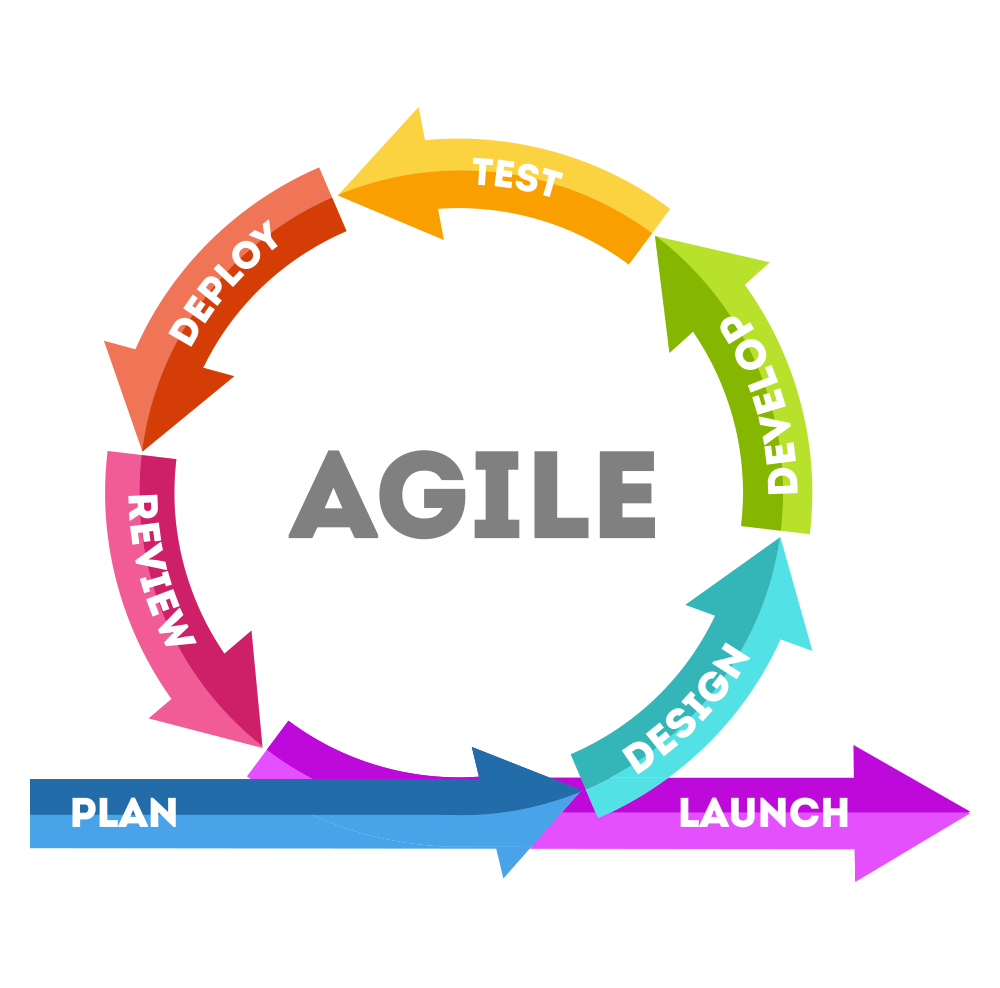
\includegraphics[alt={Agile}, width=.5\columnwidth]{thesis/files/img/metodo_agile.png}
    \caption[Struttura generale di un processo Agile.]{Struttura generale di un processo Agile. \\ \textit{fonte: \url{https://www.josoft.it/sviluppo-software-personalizzato/}}}
    \label{fig:Agile}
\end{figure} 

In particolare VisioneImpresa applica il \textit{framework} Scrum, uno dei modelli più utilizzati nell'ambito Agile. Scrum prevede la suddivisione di un periodo lungo in \textit{sprint} dalla durata fissa, di solito di 1-2 settimane, ognuno dei quali ha i propri obiettivi specifici e mira ad apportare un incremento al progetto.
L'immagine seguente mostra la struttura tipica del ciclo Scrum \ref{fig:Scrum}.

\begin{figure}[H]
    \centering
    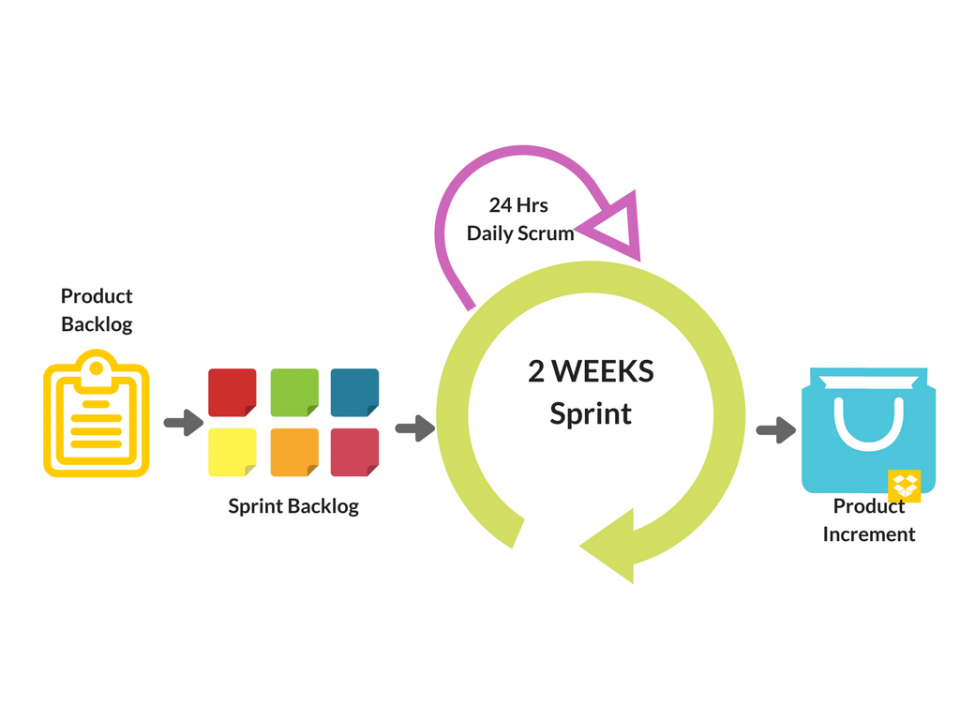
\includegraphics[alt={Scrum}, width=1\columnwidth]{thesis/files/img/Differenza-tra-Sprint-e-Sprint-Backlog-nella-metodologia-Agile-960x720.png}
    \caption[Ciclo di lavoro generale secondo Scrum.]{Ciclo di lavoro generale secondo Scrum. \\ \textit{fonte:\url{https://vitolavecchia.altervista.org/differenza-tra-sprint-e-sprint-backlog-nella-metodologia-agile/}}}
    \label{fig:Scrum}
\end{figure} 

Il \textit{framework} sopra presentato definisce un insieme di ruoli, ed eventi, così come descritti nella \textit{Scrum Guide} \footcite{misc:Guida-Scrum}. \\
Tuttavia, nel contesto di VisioneImpresa l'approccio Scrum non viene seguito in modo scolastico ma viene adottato con coerenza in alcuni casi specifici. 
In particolare, ho avuto modo di osservare direttamente la metodologia con il quale questo \textit{framework} viene applicato al progetto pluriennale di riscrittura del sistema gestionale VisionENTERPRISE, di cui fornirò più informazioni nella sotto-sezione \ref{Propensione-all'-innovazione}.
L'approccio adottato in questo contesto mantiene i principi fondamentali di questo metodo di lavoro, quali collaborazione, \textit{feedback}, trasparenza, ma presenta alcune personalizzazioni legate alle esigenze aziendali. \\
L'applicazione concreta del metodo si può riassumere nei seguenti punti:

\begin{itemize}
    \item \textbf{\textit{Sprint meeting} settimanali:}
    ogni mercoledì viene organizzata una riunione tecnica a cui partecipano gli sviluppatori coinvolti nel progetto. Questo incontro svolge sia la funzione di \textit{sprint planning} dove si discute degli obiettivi e delle funzionalità da implementare nel prossimo periodo, ma anche la funzione di \textit{sprint review} dove viene visualizzato il lavoro svolto nel periodo passato valutandone gli obiettivi conseguiti. Questa riunione viene fatta con l'obiettivo di discutere delle problematiche incontrate e fissare gli obiettivi per il prossimo periodo.
    \item \textbf{\textit{Daily meeting}:}
    ogni giorno gli sviluppatori partecipano a una breve \textit{call}, posizionata durante la mattinata, durante la quale tutti espongono cosa hanno fatto nel giorno precedente e quello in cui si concentrerà nella giornata corrente. Questo incontro viene svolto nel \textit{software} 3CX, il centralino telefonico usato per le comunicazioni interne, ed è fondamentale per mantenere tutto il \textit{team} allineato.
    \item \textbf{Flessibilità del lavoro:} 
    un'altra caratteristica osservata è che gli sviluppatori non hanno un carico di lavoro uniforme ma vengono destinate alla realizzazione del progetto, per motivi aziendali, risorse limitate, infatti lavorano a questo progetto solo alcuni giorni della settimana. Questa scelta è motivata dall'impossibilità di interrompere le attività e i processi legati al vecchio \textit{software}. Per questo motivo il \textit{team} deve gestire il lavoro con grande flessibilità per evitare blocchi o disallineamenti che rappresentano un rischio per lo sviluppo.
    \item  \textbf{Riunione mensile aziendale:}
    oltre alle attività settimanali, VisioneImpresa organizza un \textit{meeting} mensile a cui partecipano tutti i membri dell'azienda. Durante questo incontro vengono presentati gli avanzamenti conseguiti durante il mese, si fa il punto della situazione riguardante lo stato dei progetti in corso e si presenta quello che verrà fatto nel prossimo mese. Oltre a un compito di allineamento, questa riunione serve anche per favorire il dialogo tra tutti i componenti dell'azienda, i dipendenti infatti sono invitati a proporre soluzioni a eventuali problemi che sono stati individuati, avanzare idee e offrire punti di riflessione utili allo sviluppo dei progetti, sia attuali che futuri. Questa fase può essere vista come una sessione di \textit{brainstorming} aziendale dove viene stimolato un confronto sui temi trattati.
\end{itemize}
Per concludere, l'adozione del modello Scrum da parte di VisioneImpresa non segue una struttura rigida, ma si configura secondo le esigenze progettuali. Nonostante tutto questo processo, visto da un occhio esterno, risulta coerente con i principi fondamentali e si dimostra efficace nell'organizzare e coordinare un progetto di grandi dimensioni come questo.


\subsection{Tecnologie e strumenti utilizzati}
Nel contesto di competenza nel quale opera, VisioneImpresa utilizza un ampia \textit{gamma} di tecnologie a supporto delle attività. Questi strumenti possono essere divisi in base al contesto di utilizzo ovvero: strumenti operativi, strumenti per la comunicazione e la produttività, strumenti per lo sviluppo \textit{software}, strumenti per la gestione del codice e dei progetti.
Essendo così grande il numero di tecnologie impiegate e non essendo entrato in contatto con tutti gli ambiti dell'azienda, le tecnologie descritte in seguito sono solo quelle che ho avuto modo di osservare o quelle con cui ho avuto il modo di interagire durante il periodo di \textit{stage}.

\textbf{Strumenti operativi}
\begin{itemize}
  \item Portatili aziendali: ad ogni dipendente viene fornito un portatile personale, con sistema operativo Windows 10 o 11, oppure macOS. 
  \item Dispositivi mobili: per i dipendenti che si occupano di sviluppo di applicazioni \textit{mobile} vengono dati in dotazione \textit{smartphone} e/o \textit{tablet} con sistemi Android o IOS, utilizzati principalmente per funzioni di \textit{testing} delle applicazioni.
\end{itemize}

\textbf{Strumenti per la comunicazione e la produttività}
\begin{itemize}
  \item Microsoft Office 365: \textit{suite} di strumenti Microsoft per la produttività.
  \item Outlook: client integrato, facente parte della \textit{suite} Office, utilizzato per la posta elettronica e per la comunicazione interna e esterna.
  \item 3CX: centralino telefonico \mygls{PBX}, una tecnologia che consente creare una rete di comunicazioni interna, utilizzato per le chiamate vocali, messaggistica istantanea e riunioni online. 
\end{itemize}

\textbf{Strumenti per lo sviluppo \textit{software}}
\begin{itemize}
  \item Visual Studio: Un \mygls{IDE} un ambiente di sviluppo che contiene strumenti per scrivere e testare codice progettato da Microsoft. Molto utilizzato nei progetti che coinvolgono il \textit{framework} .NET , data una larga \textit{gamma} di strumenti offerti.
  \item Visual Studio Code: \textit{editor} di codice sorgente \textit{open-source}, sviluppato da Microsoft, viene contraddistinto per la sua leggerezza, velocità e personalizzazione.
  \item SQL Server Management Studio (SSMS): Questo strumento è dedicato alla gestione dei \textit{database} relazionali basati su SSMS, ha un interfaccia molto esplicativa e viene utilizzato per la gestione in tempo reale dei dati.
  \item Swagger: Piattaforma per la progettazione e la documentazione di \mygls{API} \mygls{REST}, ovvero interfacce che permettono la comunicazione tra sistemi \textit{web}, permette di visualizzare in maniera chiara le chiamate, e offre strumenti per testare le richieste e le risposte.
\end{itemize}
\textbf{\textit{Framework} e linguaggi}
\begin{itemize}
  \item .NET: Un \textit{framework} di sviluppo \textit{software} creato da Microsoft che consente lo sviluppo di vari applicazioni sia a livello \textit{desktop} sia a livello \textit{mobile} e \textit{web}. 
  \item FoxPro: Linguaggio di programmazione e sistema per la gestione del \textit{database}, attualmente considerato \textit{\mygls{legacy}} a causa della dismissione ufficiale del supporto da parte di Microsoft nel 2015. Viene utilizzato per la manutenzione in attesa della completa migrazione verso tecnologie più moderne.
\end{itemize}

\textbf{Gestione del codice e dei progetti}
\begin{itemize}
  \item Bitbucket: Strumento utilizzato per il versionamento del codice e facilitare la collaborazione tra membri del \textit{team}. Offre funzionalità di controllo delle modifiche e revisione del codice. 
  \item Jira: Strumento sviluppato da Atlassian per la gestione dei progetti e la divisione delle \textit{task}. Supporta le metodologie Agile consentendo la gestione del lavoro in \textit{sprint}.
  \item Excel: Nonostante sia uno strumento che non offre le stesse potenzialità di altri come Jira, viene utilizzato per la pianificazione elementare delle attività.
\end{itemize}

\textbf{Integrazione delle tecnologie nei processi aziendali} \\
Durante il periodo di \textit{stage} ho potuto osservare come gli strumenti e le tecnologie vengono integrate all'interno del flusso di lavoro. Nello schema seguente \ref{fig:strumenti-integrazione} viene rappresentato in maniera semplificata l'integrazione dei principali strumenti all'interno dei processi aziendali, come osservato durante la mia esperienza.

\begin{figure}[H]
\centering
\begin{tikzpicture}[
    box/.style={
        draw, rectangle,
        text width=3.4cm, align=center,
        minimum height=1.2cm, font=\small
    },
    arrow/.style={thick, ->, >=Stealth},
    node distance=1.2cm and 1.4cm
]

% Riga superiore
\node[box] (doc) {Documentazione\\\textbf{Word, Excel}};
\node[box, right=of doc] (comm) {Comunicazione\\\textbf{3CX, \\Outlook, Teams}};
\node[box, right=of comm] (task) {Gestione Attività\\\textbf{Jira, Excel}};

% Nodo centrale
\node[box, below=1.4cm of comm, text width=9cm, minimum height=2.4cm] (dev) {
\textbf{Sviluppo \textit{software}}\\
.NET, C\# $\rightarrow$ Visual Studio / VS Code\\
SQL Server $\rightarrow$ SQL Server Management Studio\\
API Testing: Swagger
};

% Frecce principali verso sviluppo
\draw[arrow] (doc.south) -- ([xshift=-2.5cm]dev.north);
\draw[arrow] (comm.south) -- (dev.north);
\draw[arrow] (task.south) -- ([xshift=2.5cm]dev.north);

% Nuove frecce laterali da "Comunicazione"
\draw[arrow, bend left=20] (comm.west) to (doc.east);
\draw[arrow, bend right=20] (comm.east) to (task.west);

% Nodo inferiore
\node[box, below=1.2cm of dev] (versioning) {Controllo Versione\\\textbf{Bitbucket (Git)}};
\draw[arrow] (dev.south) -- (versioning.north);

\end{tikzpicture}
\caption[Schema di integrazione degli strumenti nei processi aziendali]{
Schema semplificato dell'integrazione degli strumenti principali nei processi aziendali.
}
\label{fig:strumenti-integrazione}
\end{figure}

Di seguito è presentato nel dettaglio come ciascun processo aziendale viene affiancato e supportato dalle tecnologie citate.

\begin{itemize}

    \item \textbf{Documentazione} \\
    La scrittura della documentazione avviene principalmente attraverso Microsoft Word, con il quale vengono redatti i documenti più significativi, come le analisi dei requisiti e i casi d'uso, solitamente questa attività viene svolta dal responsabile di progetto e in seguito i documenti vengono condivisi con il \textit{team} di sviluppo. Nel mio periodo di \textit{stage}, ho preso visione di diversi documenti e ne ho scritti alcuni. Inoltre, vengono prodotti anche i documenti a supporto delle riunioni, che svolgono il ruolo di verbali, riportando i temi trattati. L'utilizzo di Excel si limita ad alcuni casi specifici.
    
    \item \textbf{Comunicazione} \\
    Lo strumento principale per quanto riguarda la comunicazione interna è 3CX, utilizzato per chiamate, messaggi istantanei e riunioni. È lo strumento preferito per la collaborazione rapida tra i membri dell'azienda. Io non ho avuto un account per l'accesso a 3CX e ho comunicato con Microsoft Outlook, utilizzandolo per mandare e leggere mail e messaggi. In alcune occasioni come la riunione aziendale mensile viene utilizzato Microsoft Teams .


    \item \textbf{Gestione attività} \\
    Le attività inerenti ai progetti vengono tracciate utilizzando principalmente Jira, ma talvolta a livello di supporto viene impiegato anche Microsoft Excel per via della sua semplicità. Durante il mio \textit{stage} i miei compiti erano assegnati via email o tramite riunioni in presenza, non ho utilizzato quindi in prima persona strumentazione per la gestione delle attività.

    \item \textbf{Sviluppo \textit{software}} \\
    Per quanto riguarda lo sviluppo \textit{software} le tecnologie e i linguaggi adottati variano in base al progetto di riferimento. Per la mia esperienza il \textit{framework} di riferimento è .NET, utilizzato con il linguaggio C\#, viene usato per lo sviluppo di applicazioni \textit{web} e \textit{desktop} in maniera performante. Gli ambienti di sviluppo variano sempre in base al progetto di riferimento ma principalmente vengono utilizzati Visual Studio o Visual Studio Code. Tutte le applicazioni sviluppate si interfacciano con \textit{database} relazionali gestiti tramite SQL Server Management Studio (SSMS), questo strumento viene utilizzato per la creazione, la manutenzione e l'interrogazione del \textit{database}.
    Per quanto riguarda le \mygls{API} \mygls{REST}, VisioneImpresa utilizza Swagger come strumento di testing e documentazione, favorendo la visualizzazione dei risultati e migliorando lo sviluppo.

    \item \textbf{Controllo versione} \\
    Per quanto riguarda invece la gestione del codice in azienda viene utilizzato Bitbucket. Anche se non mi sono interfacciato direttamente con i \textit{repository}, ho visualizzato alcuni flussi tipici del codice. Il codice di ogni progetto viene messo in \textit{repository} dedicati, i quali poi sono strutturati in \textit{branch} come \textit{main}, \textit{develop} e \textit{branch} specifici per implementare funzionalità.
    Questo strumento consente di mantenere il codice stabile e versionato, migliorando lo sviluppo in parallelo.
   
\end{itemize}

\section{Propensione all'innovazione}
\label{Propensione-all'-innovazione}
VisioneImpresa non dispone di un reparto dedicato alla ricerca e sviluppo, ciononostante l'innovazione e l'aggiornamento rappresentano un elemento fondamentale sulla quale si basa la filosofia aziendale. 
Essendo un'azienda che opera da oltre quarant'anni nel settore dell'\textit{Information Technology}, ha avviato un processo di transizione tecnologica di ampio raggio, tra le iniziative più significative c'è la progressiva migrazione dei sistemi \mygls{ERP} sviluppati in FoxPro verso ambienti più moderni e performanti. Questo processo per complessità e dimensione richiede una pianificazione pluriennale e il coinvolgimento graduale di un gran numero di risorse.
In parallelo a questa transizione, VisioneImpresa considera i progetti di \textit{stage} un'opportunità concreta per il progresso. Durante il mio tirocinio, ho avuto modo di contribuire attivamente allo sviluppo di progetti finalizzati alla modernizzazione. In particolare mi è stato comunicato che uno dei due progetti a cui ho avuto modo di lavorare è destinato a integrarsi con il nuovo gestionale attualmente in fase di sviluppo, pensato per sostituire l'attuale \mygls{ERP} con una soluzione più moderna e tecnologicamente avanzata.
Inoltre, l'azienda incoraggia gli stagisti a proporre nuove idee e soluzioni tecniche, introducendo anche nuove tecnologie in autonomia. Questa libertà consente di testare nuove soluzioni in un ambiente controllato, favorendone la possibile introduzione nei processi aziendali.

\newpage